\documentclass[border=8pt]{standalone}
% For a normal document use: \documentclass{article} + \usepackage{tikz}
\usepackage{tikz}
\usepackage{amsmath}
\usetikzlibrary{fit,positioning,arrows.meta,calc}

%========================= shared styles =========================
\tikzset{
  latent/.style = {circle, draw, thick, minimum size=10mm, inner sep=1pt},
  obs/.style    = {circle, draw, thick, fill=black!10, minimum size=10mm, inner sep=1pt},
  par/.style    = {rectangle, draw, thick, rounded corners=2pt,
                   minimum height=7.5mm, inner sep=4pt},
  hyper/.style  = {rectangle, draw, thick, fill=black, minimum size=2.4mm, inner sep=0pt},
  plate/.style  = {rectangle, draw, dashed, rounded corners=3pt, inner sep=7mm},
  edge/.style   = {-{Stealth[length=2.5mm]}, thick},
  lab/.style    = {font=\small, inner sep=1.5pt},
  note/.style   = {font=\footnotesize\itshape, inner sep=1.5pt},
}

\begin{document}

%================================================================
% FIGURE 1 --- flat prior on mu
%================================================================
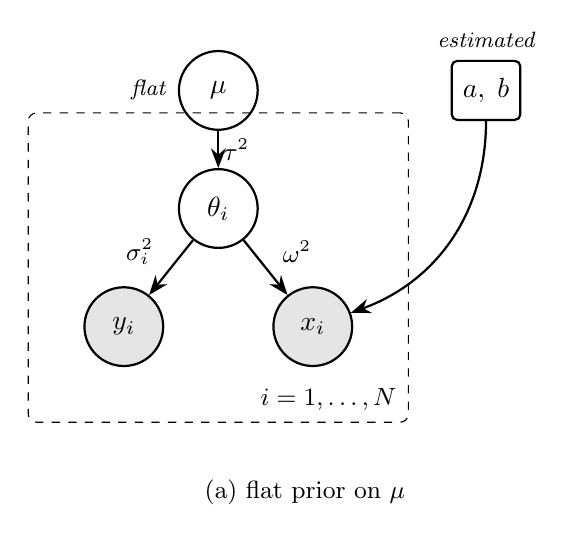
\begin{tikzpicture}

  \node[latent] (mu) at (0,3)     {$\mu$};
  \node[latent] (th) at (0,1.5)   {$\theta_i$};
  \node[obs]    (y)  at (-1.2,0)  {$y_i$};
  \node[obs]    (x)  at (1.2,0)   {$x_i$};
  \node[par]    (ab) at (3.4,3)   {$a,\;b$};

  % plate over the units
  \node[plate, fit=(th)(y)(x)] (pl) {};
  \node[anchor=south east, lab] at ($(pl.south east)+(-1mm,1mm)$) {$i=1,\dots,N$};

  % edges
  \draw[edge] (mu) -- node[lab, right] {$\tau^2$} (th);
  \draw[edge] (th) -- node[lab, pos=.5, xshift=-4mm, yshift=2mm] {$\sigma_i^2$} (y);
  \draw[edge] (th) -- node[lab, pos=.5, xshift=4mm, yshift=2mm] {$\omega^2$}   (x);
  \draw[edge] (ab) to[out=-90, in=20] (x);

  % annotations
  \node[note, left=1mm of mu]  {flat};
  \node[note, above=1mm of ab] {estimated};
  \node[font=\small] at (1.1,-2.1) {(a) flat prior on $\mu$};

\end{tikzpicture}
\qquad

%================================================================
% FIGURE 2 --- proper prior  mu ~ N(0, sigma_mu^2)
%================================================================
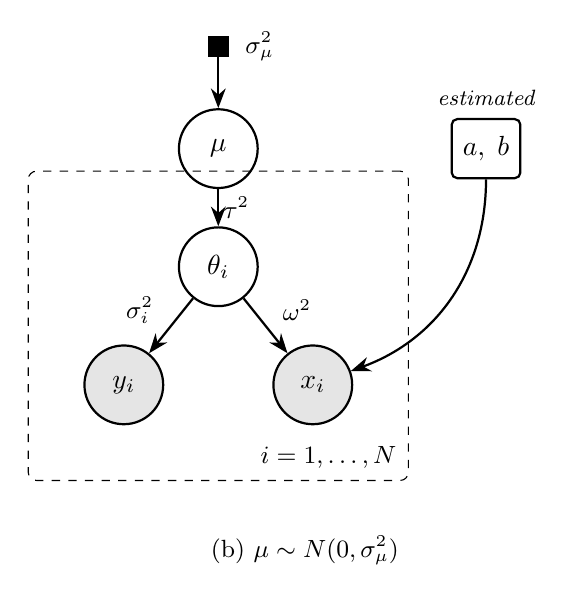
\begin{tikzpicture}

  \node[hyper]  (sm) at (0,4.3)   {};
  \node[lab, right=1.5mm of sm]   {$\sigma_\mu^2$};
  \node[latent] (mu) at (0,3)     {$\mu$};
  \node[latent] (th) at (0,1.5)   {$\theta_i$};
  \node[obs]    (y)  at (-1.2,0)  {$y_i$};
  \node[obs]    (x)  at (1.2,0)   {$x_i$};
  \node[par]    (ab) at (3.4,3)   {$a,\;b$};

  \node[plate, fit=(th)(y)(x)] (pl) {};
  \node[anchor=south east, lab] at ($(pl.south east)+(-1mm,1mm)$) {$i=1,\dots,N$};

  \draw[edge] (sm) -- (mu);
  \draw[edge] (mu) -- node[lab, right] {$\tau^2$} (th);
  \draw[edge] (th) -- node[lab, pos=.5, xshift=-4mm, yshift=2mm] {$\sigma_i^2$} (y);
  \draw[edge] (th) -- node[lab, pos=.5, xshift=4mm, yshift=2mm] {$\omega^2$}   (x);
  \draw[edge] (ab) to[out=-90, in=20] (x);

  \node[note, above=1mm of ab] {estimated};
  \node[font=\small] at (1.1,-2.1) {(b) $\mu\sim N(0,\sigma_\mu^2)$};

\end{tikzpicture}

\end{document}
